\documentclass[12pt]{article}
\usepackage[left=1in, right=1in, top=1in, bottom=1in]{geometry}
\usepackage{amsmath, amssymb, amsfonts}
\usepackage{graphicx}
\usepackage{xcolor}
\usepackage{float}
\usepackage{booktabs}

\begin{document}
	\begin{center}
	{\Large Mitigation model}	
	\end{center}
	
	\section{State variables and law of motion}
	
	Total capital:
	$$
	d \log K = (\mu_k + i - \frac{\kappa}{2} i^2 - \frac{\sigma_k^2}{2}) dt + \sigma_k dW
	$$
	
	Temperature anomaly:
	$$
	d Y = e(\theta_\ell dt + \varsigma dW)
	$$
	
	$R\& D$ investment, $X$, leads to an increased arrival rate of a one time jump in green sector productivity:
	$$
	d\log \mathcal{I}_g = - \zeta dt + \Psi_0 (\frac{X}{\mathcal{I}_g})^{\Psi_1} dt - \frac{\sigma_g^2}{2} dt + \sigma_g dW 
	$$
	
	Here we use $\Psi_1 = 1/2$
	\section{Pre-damage and pre technology jump HJB}
	Denote $x = \frac{X}{K}$ as R\& D invesment - total capital ratio, and there are two technology jumps. The pre damage jump and pre technology jump HJB:
	\begin{align*} 
		0 = \max_{i,e,x} \min_{\omega_\ell, \sum_{\ell = 1}^L \omega_\ell = 1, g, g_m } &   - \delta V(\log K,Y, \log \mathcal{I}_g) +  \delta \log \left( \alpha - i -  \alpha \overline{\vartheta} \left[ 1 - \left(\frac {e} { \alpha \overline\lambda K} \right) \right]^\theta  - x \right) + \delta\log K \cr 
		& + \frac {\partial V}{\partial \log K} 
		\left[ \mu_k    + i   -
		{\frac { \kappa} 2} i^2  -  \frac  {|\sigma_k|^2}  2\right]  + \frac {|\sigma_k|^2} 2  \frac {\partial^2 V}{\partial \log K^2} \cr
		& + \frac {\partial  V(\log K,Y)}{\partial Y}  \sum_{\ell=1}^L \omega_\ell  \theta_\ell {e} + {\frac 1 2} \frac {\partial^2 V}{\partial Y^2} |\varsigma|^2 e^2  \cr
		& - \left( \left[ \gamma_1 + \gamma_2 Y\right]   \sum_{\ell=1}^L \omega_\ell \theta_\ell { e} + {\frac 1 2} (\gamma_2 ) |\varsigma|^2  e^2 \right) \cr
		& + \frac{\partial V}{\partial \log \mathcal{I}_g} (- \zeta + \Psi_0 x^{\Psi_1} - \frac{\sigma_g^2}{2} ) + \frac{\sigma_g^2}{2}\frac{\partial^2 V}{\partial \log \mathcal{I}_g^2} \\
		& + \xi_a \sum_{\ell = 1}^L \omega_\ell \left( \log \omega_\ell - \log \pi_\ell \right) \\
		& + \xi_g \mathcal{I}_g \left(1 - g + g  \log(g) \right) + \mathcal{I}_g g (V^{\text{post tech, m}} - V )\\
		& + \sum_{m=1}^M \pi_d^m g_m (V^m - V) + \xi_d \sum_{m=1}^M \pi_d g_m (1 - g_m + g_m \log(g_m))
	\end{align*} 
	
	\section{Uncertainty parameter configuration}
	\begin{itemize}
		\item Smooth ambiguity: $\xi_a$
		\item Damage uncertainty, $\xi_d$,
		\item Technology jump uncertainty, $\xi_g$
	\end{itemize}
	
	\begin{table}[H]
		\centering
		\begin{tabular}{llll}
			\toprule
			& $\xi_a$ & $\xi_d$ & $\xi_g$ \\
			\midrule
			baseline & $\infty$ & $\infty$ & $\infty$\\
			case 1 & $2 \times 10^{-4}$ & 0.050 & 0.050 \\
			case 2 & $2 \times 10^{-4}$ & 0.025& 0.025\\
			\bottomrule
		\end{tabular}
	\end{table}

\section{Pathway comparisons, with 20 damage functions}

\subsection{pre damage jump, pre technology jump R\& D investment}
\begin{figure}[H]
	\centering
	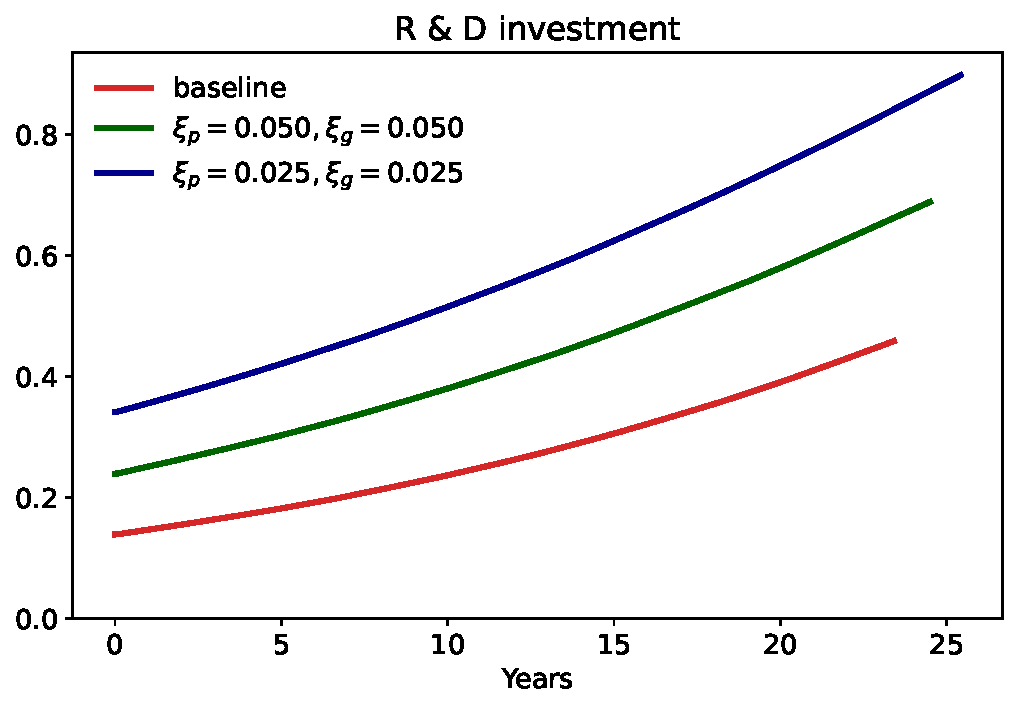
\includegraphics[width=\textwidth]{../figures/xi_comparison/20damage/Xt_1p5.pdf}
	\caption{R \& D investment, pathways stop when temperature anomaly hits $1.5^o C$}
\end{figure}

\subsection{pre damage jump, pre technology jump emission}
\begin{figure}[H]
	\centering
	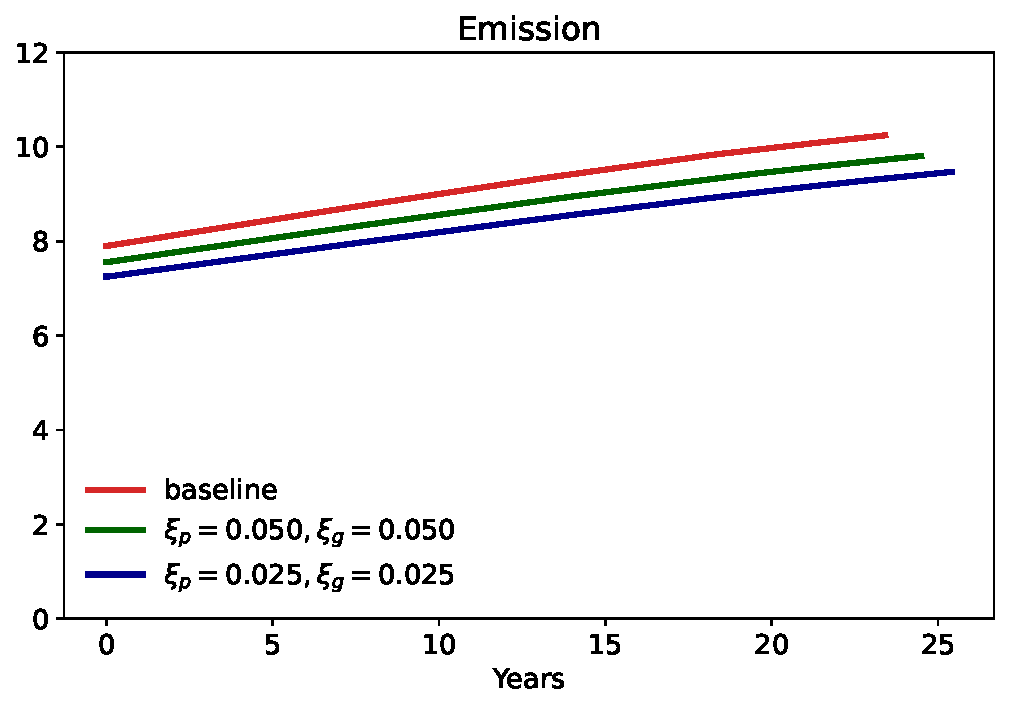
\includegraphics[width=\textwidth]{../figures/xi_comparison/20damage/Et_1p5.pdf}
	\caption{Emission, pathways stop when temperature anomaly hits $1.5^o C$}
\end{figure}

\subsection{pre damage jump, pre technology jump temperature anomaly}
\begin{figure}[H]
	\centering
	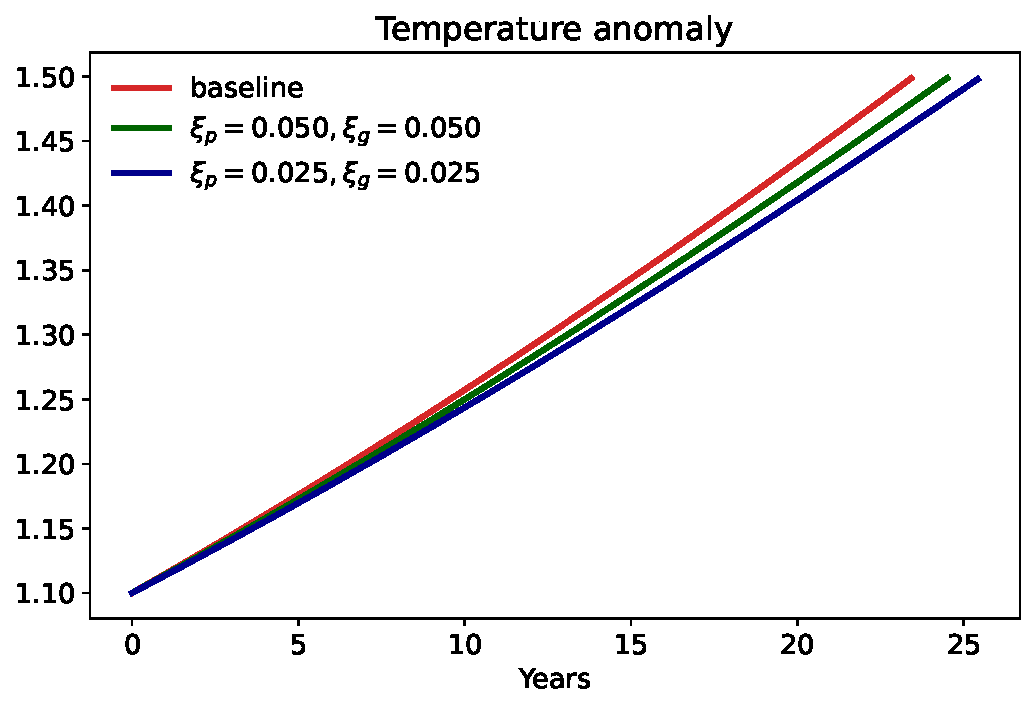
\includegraphics[width=\textwidth]{../figures/xi_comparison/20damage/Yt_1p5.pdf}
	\caption{Temperature anomaly, pathways stop when temperature anomaly hits $1.5^o C$}
\end{figure}

\subsection{pre damage jump, pre technology jump technology jump intensity, $\mathcal{I}_g$}
\begin{figure}[H]
	\centering
	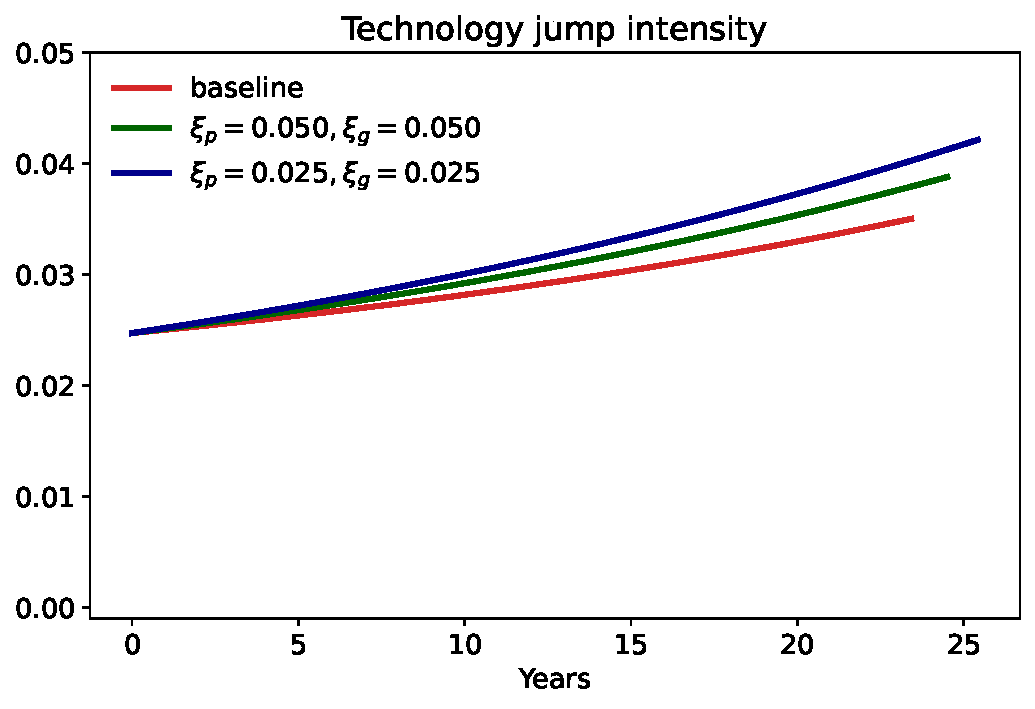
\includegraphics[width=\textwidth]{../figures/xi_comparison/20damage/Lt_1p5.pdf}
	\caption{Technology jump intensity, $\mathcal{I}_g$, pathways stop when temperature anomaly hits $1.5^o C$}
\end{figure}

\section{Jump probabilities and distorted probabilities}

\subsection{Distorted probability of Poisson events for technology changes with different uncertainty configurations}


\begin{figure}[H]
	\centering
	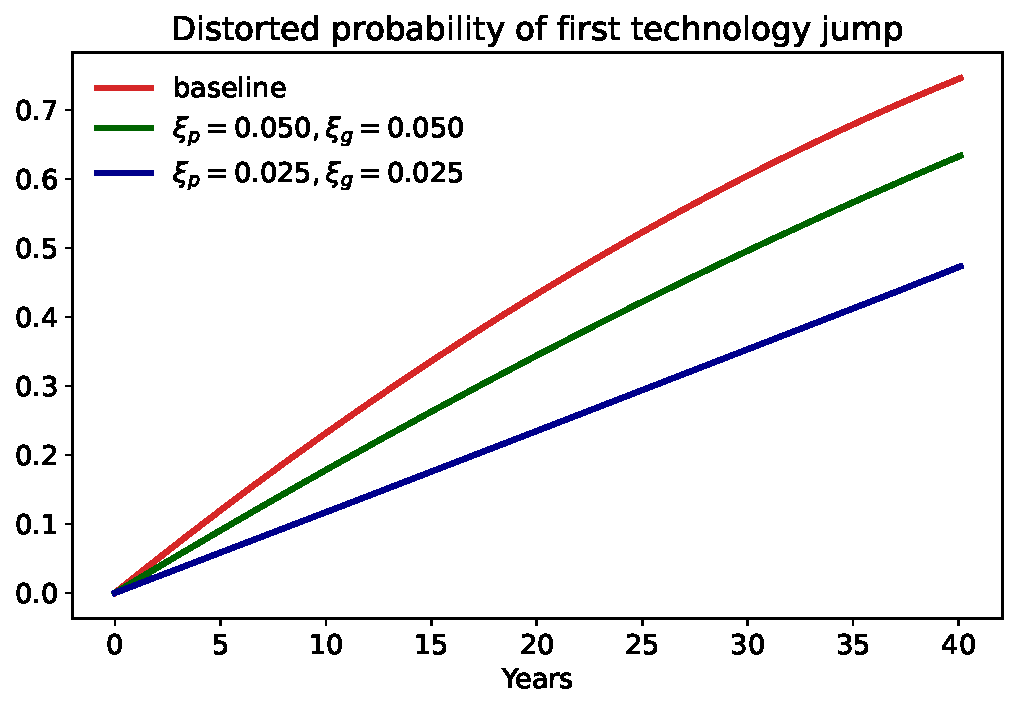
\includegraphics[width=0.85\textwidth]{../figures/xi_comparison/20damage/Tech_jump_first.pdf}
\end{figure}

\begin{figure}[H]
	\centering
	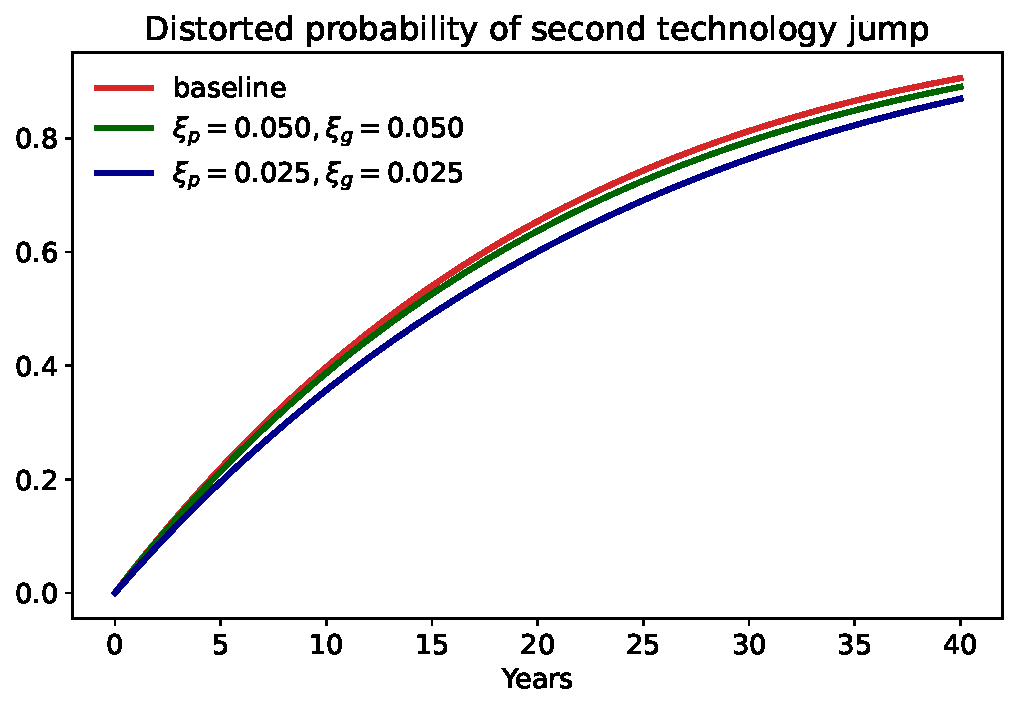
\includegraphics[width=0.85\textwidth]{../figures/xi_comparison/20damage/Tech_jump_second.pdf}
\end{figure}

\subsection{Distorted probability of Poisson events for damage with different uncertainty configurations}


\begin{figure}[H]
	\centering
	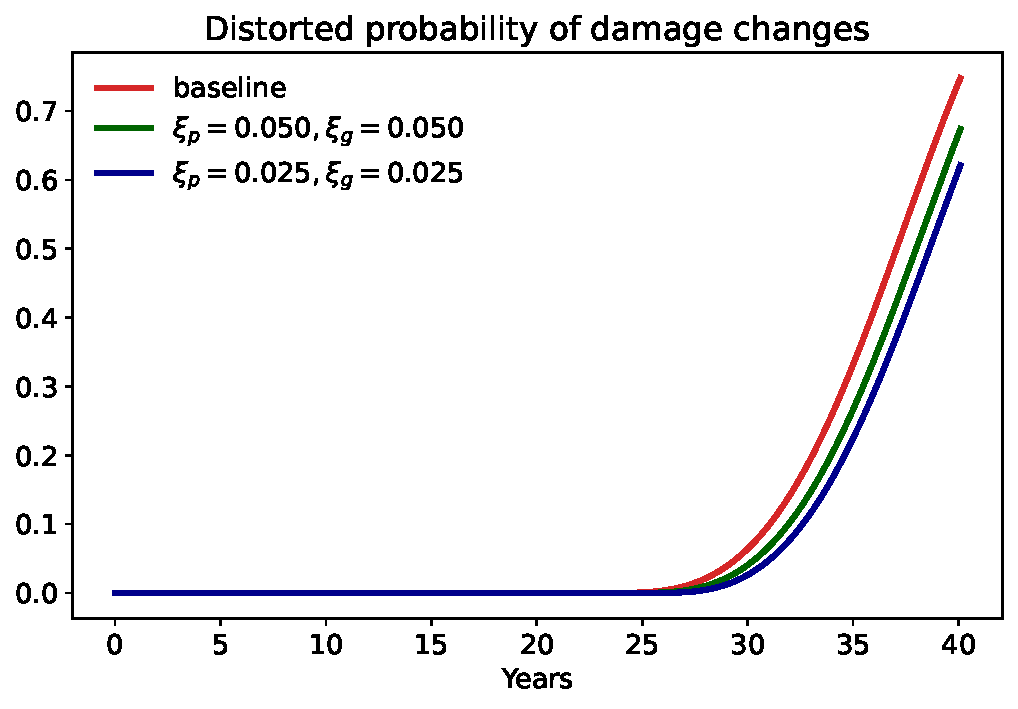
\includegraphics[width=0.85\textwidth]{../figures/xi_comparison/20damage/Damage_prob.pdf}
\end{figure}

\subsection{Probability distortion for damage function, with $\xi_a = 2\times 10^{-4}$, $\xi_d = 0.05$ and $\xi_g = 0.05$}

\begin{figure}[H]
	\centering
	\includegraphics[width=0.85\textwidth]{../figures/xi_comparison/20damage/Damage_distort.pdf}
	\caption{Red bars are for baseline probability, and blue bars are for distorted probability}
\end{figure}

\subsection{Probability distortion for climate sensitivity models, with $\xi_a = 2\times 10^{-4}$, $\xi_d = 0.05$ and $\xi_g = 0.05$}

\begin{figure}[H]
	\centering
	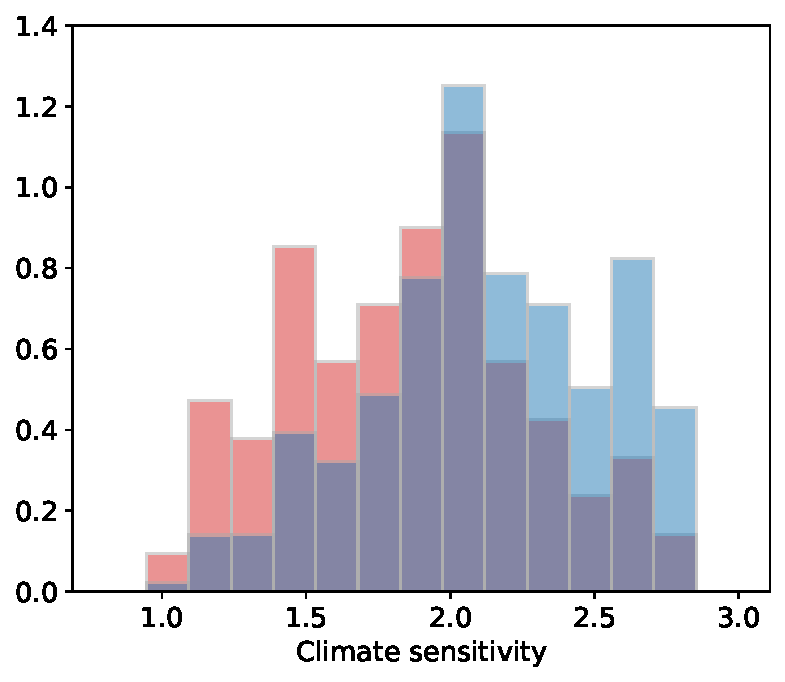
\includegraphics[width=0.85\textwidth]{../figures/xi_comparison/20damage/worstcase.pdf}
		\caption{Red bars are for baseline density, and blue bars are for distorted density of climate sensitivity models}
\end{figure}
\end{document}